\chapter{Network Diagram}
% Set Pagestyle to Fancy
\pagestyle{fancy}

% Clear all header and footer fields
\fancyhf{}

% Page number only in the center of the footer
\fancyfoot[C]{\thepage}

% Remove header line
\renewcommand{\headrulewidth}{0pt}
\renewcommand{\footrulewidth}{0pt}

\section{Purpose}
The purpose of the Network Diagram section is to establish clear guidelines and requirements for the creation, maintenance, and protection network diagram information/infrastructure. Accurate network diagrams are critical to understanding our organization's IT infrastructure, facilitating trouble shooting, maintenance, information relevant to incident response, and validating compliance with security standards and regulations. Following the guidelines of this policy ensures that all network diagrams accurately represent the current state of Honda Motor Co., Ltd. network, including all operation critical systems, devices, communication links, and security boundaries. Not only this but this policy defines how these diagrams must be classified, stored, and shared to prevent unauthorized access and protect sensitive information. By enforcing a structured and secure approach to diagram management, the organization reduces the risk of threats, enhances incident recovery efficiency, and supports ongoing network audits and compliance efforts.
\section{Scope}
The policies regarding the network diagram are subject to any/all persons or groups that have access to the network diagram and infrastructure data. This includes network and system administrators, IT staff, contractors, and third-party vendors who design, modify, or manage network infrastructure across all corporate, manufacturing, and affiliated sites globally. operational sites or facilities that are subject to policies regarding network diagram are as follows
\begin{itemize}
    \item Corporate headquarters, regional offices, and administrative sites
    \item Manufacturing plants, warehouses, and other industrial facilities
    \item Dealership, retail outlets, and service centers under Honda Motor Co., Ltd. management
    \item Company operated data centers, cloud environments (hybrid or other included)
    \item Remote access infrastructure for employees, contractors, and mobile staff
    \item Third-party sites with integrated network access
    \item international or cross-border facilities connected to the company network
\end{itemize}

\section{Policy requirements}
This section highlights the mandatory requirements for the creation, classification, maintenance, and use of network diagrams throughout Honda Motor Co., Ltd.
\begin{itemize}
    \item \textbf{Accuracy and completeness:} All network diagrams and associated network infrastructure documentation are required to reflect the state of logical and physical network topologies according to the date it is recorded or created.
    \item \textbf{Key components:} Network diagrams must include business standard nomenclature along with accurate labeling. Diagrams are obligated to label key infrastructure components such as routers, switches, servers, wireless access points, VLANS, ip address ranges, cloud services, and segmentation zones.
    \item \textbf{Operational Technology and Diagram crossover:} OT environments must be diagrammed separately from network infrastructure but still integrated at crossover points (e.g., firewalls or data aggregators)
    \item \textbf{Diagram discrepancies:} Network diagrams must be updated when modifications to the network occur. When a change is instituted, network diagrams must be dated when last modified. In the event that an individual finds an incomplete, outdated, or inconsistent network diagram, the procedure is to report the discrepancies to a supervisor or administrator.
    \item \textbf{Standardization and format:} All diagrams must adhere to standardized format and notation. All diagramming tools must be company-approved. Diagrams must include accurate dates, version numbers, authors, legends, appropriate labels for zones and devices. Standardized format is required to ensure that diagrams are universally understandable across teams and departments.
    \item \textbf{Classification and access control:} All network diagrams mapping Honda Motor Co., Ltd. sites are confidential information. Informational security is critical to reducing risk. All network diagrams and associated infrastructure documentation must be stored in secure document repositories. Security controls that are to be used to control access are role-based access controls, multi-factor authentication, along with encrypted storage and transmission. Access logs must be maintained for all diagrams representing critical infrastructure
    \item \textbf{Version Control and Change management} 
    All network diagrams must include history with timestamps, authors, and edit descriptions. In the event of modification to network resources the appropriate editor must update the network within 5 business days. Any and all modifications to the network diagram must approved by the appropriate authority as well as vetted by company change control processes.
    \item \textbf{Storage, backup and retention}
    Network diagrams are subject to the Honda Motor Co., Ltd. backup policy and must be included in regular backup cycles alongside other mission-critical information assets. Network Diagrams must be retained for at least five (5) years or longer if required by regulation or audit standards. Accurate offline backups must exist for network diagrams at all sites to ensure availability during network outages, cyber incidents, or loss of primary access systems.
    \item \textbf{Incident response and emergency access}
    Network diagrams must be integrated into Honda Motor Co., Ltd. Incident Response Plan (IRP). Emergency versions must adhere to the following guidelines. Diagrams must be stored in designated security operations centers (SOCs), reasonably accessible during a declared cyber event or outage, available in both digital and physical form for high priority sites.
    \item \textbf{Review and audit}
    Network diagrams must adhere to the guidelines regarding accuracy validation. Diagrams must be certified as accurate every 6 months within corporate IT networks, every 3 months within manufacturing (OT) networks, and after any infrastructure project or re-architecture. Security and compliance teams will audit diagram management practices during internal or third-party audits.
\end{itemize}
\section{Third-Party access and sharing of network diagrams}
To preserve the confidentiality and integrity of Honda Motor Co., Ltd. network architecture, third-party access to network diagrams is strictly regulated. Due to the fact network diagrams may expose sensitive system configurations, segmentation zones, and security controls or other, any access granted to external entities must be carefully controlled and limited to only that which is strictly necessary. Prior to sharing any network diagrams with third-party entities, service providers, auditors, consultants, or other, the following requirements must be met:
\begin{itemize}
    \item \textbf{Non-disclosure agreement (NDA):}
    A legally binding and current NDA must be in place between Honda Motor Co., Ltd. and the third party. The NDA must cover the handling of network infrastructure and sensitive documentation.
    \item \textbf{Data sharing agreement}
    A data-sharing agreement must be vetted and approved by both by the legal department and information security office. this agreement must define the scope, duration, purpose, and the handling requirements for all information and documentation regarding network diagrams and infrastructure.
    \item \textbf{Role-based and scope limitations}
    Third-party access is limited to individuals whose job responsibilities necessitate direct interaction with the applicable network segment(s). Blanket access is not permitted. Shared diagrams must be limited to include only the relevant portions necessary for the third party to perform its contracted duties. Enterprise wide diagrams may not be distributed unless expressly authorized by both the chief information security officer (CISO) and legal.
    \item \textbf{Handling and Security obligations}
    All network diagrams must be communicated through secure and encrypted channels. All communicated network diagrams must be watermarked and labeled appropriately according to its classification. Third parties are not permitted to alter, replicate, or redistribute the diagrams without prior written authorization from Honda Motor Co., Ltd. Access is restricted by time, and credentials must be revoked immediately upon completion of the contractual agreement or upon termination of the agreement.
    \item \textbf{Third-party long term retention}
    Third parties are strictly prohibited from retaining permanent copies of any network diagram unless it meets the following expectations. It is explicitly required as part of the contractual engagement and written approval has been granted by the Information Security Office and Legal Department. In all other cases all copies must be returned or securely destroyed at the conclusion of the agreement, and the third party must provide documented proof of destruction upon request.
    \item \textbf{Compliance and audit}
    Third-party access to network diagrams is subject to audit by Honda Motor Co., Ltd. at any time during or after the terms of the agreement. Any violations of these terms may result in immediate termination of access, contract cancellation, and/or legal action.
\end{itemize}
\section{Enforcement}
Violations of this policy may result in disciplinary action, including access revocation, reassignment, formal reprimand, or termination of contract. In cases where violations result in regulatory non-compliance or security breaches, offenders may be reported to the appropriate internal governance bodies and/or regulatory authorities.

\section{Network Diagram}
\begin{figure}[htbp]
    \centering
    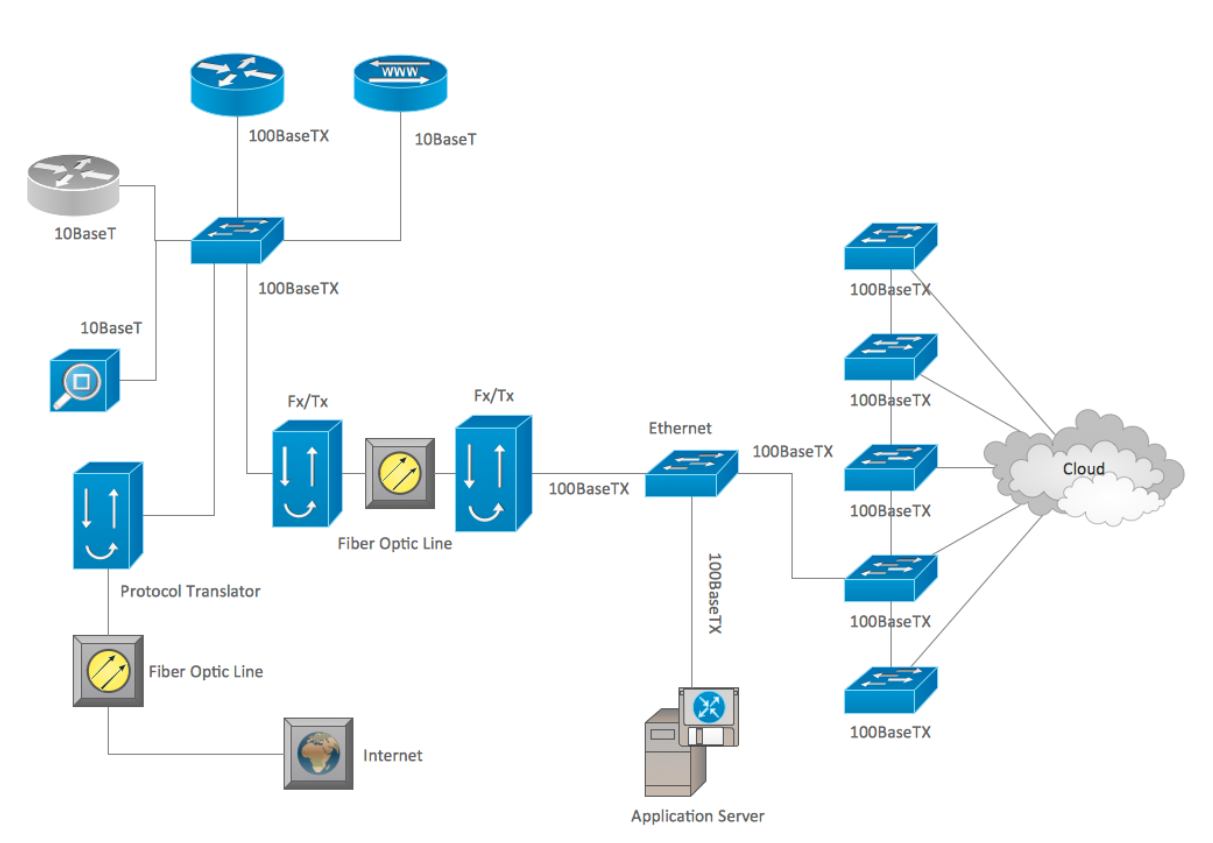
\includegraphics[width=0.8\linewidth]{images/image1.png}
    \caption{Representation similar to our company network}
    \label{fig:Diagram 7.23.2025}
\end{figure}